\lab{SQL 2 (The Sequel)}{SQL 2 (The Sequel)}
\objective{
Since SQL databases contain multiple tables, retrieving information about the data can be complicated.
In this lab we discuss joins, grouping, and other advanced SQL query concepts to facilitate rapid data retrieval.
% SQL queries can often get very complex, and can involve several relations in a database.
% In this lab, we discuss how to join tables together in order to get information stored between them.
% We also discuss several other advanced SQL selection concepts, such as: aggregate functions, ordering, grouping, case expressions, and comparison structures.
}

We will use the following database as an example throughout this lab, found in \texttt{students.db}.

\begin{table}[H]
\begin{subtable}{0.55\textwidth}
    \centering
    \begin{subtable}{.45\textwidth}
        \centering
        \footnotesize
        \begin{tabular}{|l|l|}
            \hline MajorID & MajorName \\ \hline
            1 & Math \\
            2 & Science \\
            3 & Writing \\
            4 & Art \\ \hline
        \end{tabular}
        \caption{MajorInfo}
        \label{table:sql1-student-majorinfo}
    \end{subtable}
    \hfil
    \begin{subtable}{.45\textwidth}
        \centering
        \footnotesize
        \begin{tabular}{|l|l|}
            \hline CourseID & CourseName \\ \hline
            1 & Calculus \\
            2 & English \\
            3 & Pottery \\
            4 & History \\ \hline
        \end{tabular}
        \caption{CourseInfo}
        \label{table:sql1-student-courseinfo}
    \end{subtable}
    \\[1.em] % NOTE: Use 4.01em to align the tables at the top and bottom.
    \begin{subtable}{\textwidth}
        \centering
        \footnotesize
        \begin{tabular}{|l|l|l|}
            \hline StudentID & StudentName & MajorID \\ \hline
            401767594 & Michelle Fernandez & 1 \\
            678665086 & Gilbert Chapman & NULL \\
            553725811 & Roberta Cook & 2 \\
            886308195 & Rene Cross & 3 \\
            103066521 & Cameron Kim & 4 \\
            821568627 & Mercedes Hall & NULL \\
            206208438 & Kristopher Tran & 2 \\
            341324754 & Cassandra Holland & 1 \\
            262019426 & Alfonso Phelps & NULL \\
            622665098 & Sammy Burke & 2 \\ \hline
        \end{tabular}
        \caption{StudentInfo}
        \label{table:sql1-student-info}
    \end{subtable}
\end{subtable}
\hfil
\begin{subtable}{.35\textwidth}
    \centering
    \footnotesize
    \begin{tabular}{|l|l|l|}
        \hline StudentID & CourseID & Grade \\ \hline
        401767594 & 4 & C \\
        401767594 & 3 & B-- \\
        678665086 & 4 & A+ \\
        678665086 & 3 & A+ \\
        553725811 & 2 & C \\
        678665086 & 1 & B \\
        886308195 & 1 & A \\
        103066521 & 2 & C \\
        103066521 & 3 & C-- \\
        821568627 & 4 & D \\
        821568627 & 2 & A+ \\
        821568627 & 1 & B \\
        206208438 & 2 & A \\
        206208438 & 1 & C+ \\
        341324754 & 2 & D-- \\
        341324754 & 1 & A-- \\
        103066521 & 4 & A \\
        262019426 & 2 & B \\
        262019426 & 3 & C \\
        622665098 & 1 & A \\
        622665098 & 2 & A-- \\ \hline
    \end{tabular}
    \caption{StudentGrades}
    \label{table:sql1-student-grades}
\end{subtable}
\caption{Student database.}
\end{table}

\section*{Joining Tables} % ===================================================

A \emph{join} combines rows from different tables in a database based on common attributes.
In other words, a join operation creates a new, temporary table containing data from 2 or more existing tables.
Join commands in SQLite have the following general syntax.
\begin{lstlisting}
SELECT <alias.column, ...>
    FROM <table> AS <alias> JOIN <table> AS <alias>, ...
    ON <alias.column> == <alias.column>, ...
    WHERE <condition>
\end{lstlisting}

The \lsql{ON} clause tells the query how to join tables together.
Typically if there are $N$ tables being joined together, there should be $N-1$ conditions in the \lsql{ON} clause.

\subsection*{Inner Joins} % ---------------------------------------------------

An \emph{inner join} creates a temporary table with the rows that have exact matches on the attribute(s) specified in the \lsql{ON} clause.
Inner joins \textbf{intersect} two or more tables, as in Figure \ref{fig:sql2-inner-join}.

\begin{figure}[H] % Inner and outer joins.
\captionsetup[subfigure]{justification=centering}
\centering
\begin{subfigure}{.4\textwidth}
    \centering
    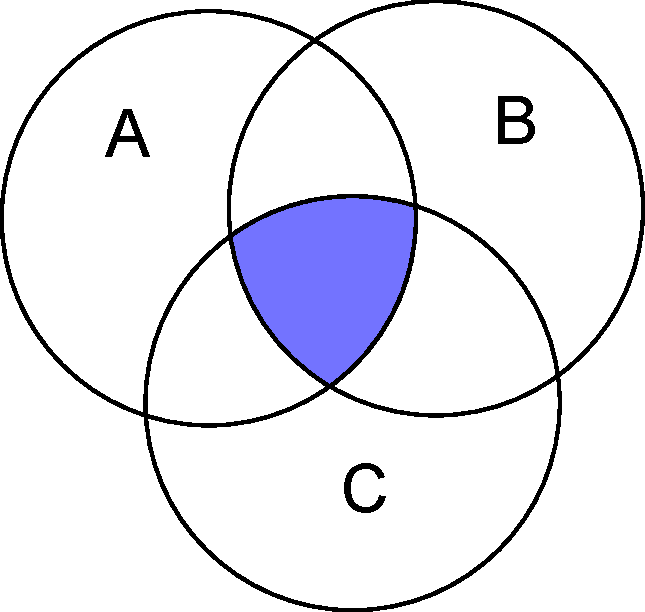
\includegraphics[width=\textwidth]{figures/inner_join.pdf}
    \caption{An inner join of A, B, and C.}
    \label{fig:sql2-inner-join}
\end{subfigure}
\hfil
\begin{subfigure}{.4\textwidth}
    \centering
    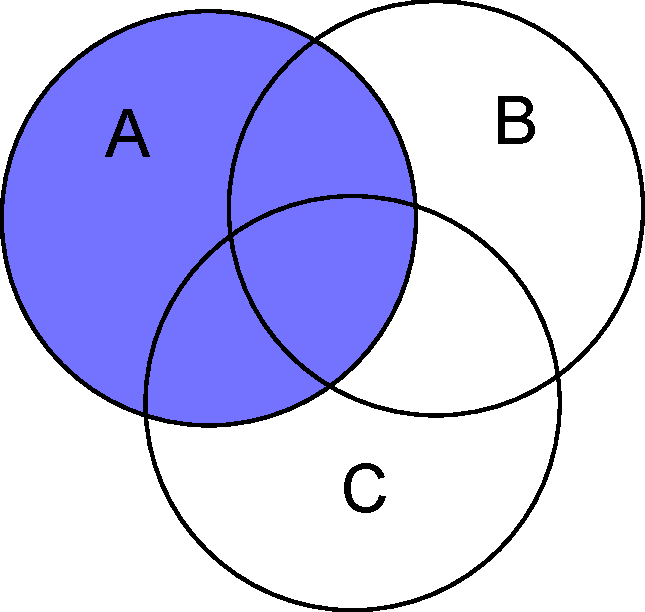
\includegraphics[width=\textwidth]{figures/left_outer.pdf}
    \caption{A left outer join of A with B and C.}
    \label{fig:sql2-left-join}
\end{subfigure}
%
% \begin{subfigure}{.3\textwidth}
%     \centering
%     \includegraphics[width=\textwidth]{figures/full_outer.pdf}
%     \caption{A full outer join of A, B, and C.}
%     \label{fig:sql2-full-join}
% \end{subfigure}
\caption{}
\label{fig:joins}
\end{figure}

For example, Table \ref{table:sql1-student-info} (\li{StudentInfo}) and Table \ref{table:sql1-student-majorinfo} (\li{MajorInfo}) both have a \li{MajorID} column, so the tables can be joined by pairing rows that have the same \li{MajorID}.
Such a join temporarily creates the following table.

\begin{table}[H]
\centering
\footnotesize
\begin{tabular}{|l|l|l|l|l|}
    \hline StudentID & StudentName & MajorID & MajorID & MajorName \\ \hline
    401767594 & Michelle Fernandez & 1 & 1 & Math \\
    % 678665086 & Gilbert Chapman & NULL \\
    553725811 & Roberta Cook & 2 & 2 & Science \\
    886308195 & Rene Cross & 3 & 3 & Writing \\
    103066521 & Cameron Kim & 4 & 4 & Art \\
    % 821568627 & Mercedes Hall & NULL \\
    206208438 & Kristopher Tran & 2 & 2 & Science \\
    341324754 & Cassandra Holland & 1 & 1 & Math \\
    % 262019426 & Alfonso Phelps & NULL \\
    622665098 & Sammy Burke & 2 & 2 & Science \\ \hline
\end{tabular}
\caption{An inner join of \li{StudentInfo} and \li{MajorInfo} on \li{MajorID}.}
\label{table:sql2-inner-join-temp}
\end{table}

Notice that this table is missing the rows where \li{MajorID} was \lsql{NULL} in the \li{StudentInfo} table.
This is because there was no match for \lsql{NULL} in the \li{MajorID} column of the \li{MajorInfo} table, so the inner join throws those rows away.

Because joins deal with multiple tables at once, it is important to assign table aliases with the \lsql{AS} command.
Join statements can also be supplemented with \lsql{WHERE} clauses like regular queries.

\begin{lstlisting}
>>> import sqlite3 as sql
>>> conn = sql.connect("students.db")
>>> cur = conn.cursor()

>>> cur.execute("SELECT * "
...             "FROM StudentInfo AS SI INNER JOIN MajorInfo AS MI "
...             "ON SI.MajorID = MI.MajorID;").fetchall()
<<[(401767594, 'Michelle Fernandez', 1, 1, 'Math'),
 (553725811, 'Roberta Cook', 2, 2, 'Science'),
 (886308195, 'Rene Cross', 3, 3, 'Writing'),
 (103066521, 'Cameron Kim', 4, 4, 'Art'),
 (206208438, 'Kristopher Tran', 2, 2, 'Science'),
 (341324754, 'Cassandra Holland', 1, 1, 'Math'),
 (622665098, 'Sammy Burke', 2, 2, 'Science')]>>

# Select the names and ID numbers of the math majors.
>>> cur.execute("SELECT SI.StudentName, SI.StudentID "
...             "FROM StudentInfo AS SI INNER JOIN MajorInfo AS MI "
...             "ON SI.MajorID = MI.MajorID "
...             "WHERE MI.MajorName == 'Math';").fetchall()
<<[('Cassandra Holland', 341324754), ('Michelle Fernandez', 401767594)]>>
\end{lstlisting}

\begin{problem} % Simple inner join.
Write a function that accepts the name of a database file.
Assuming the database to be in the format of Tables \ref{table:sql1-student-majorinfo}--\ref{table:sql1-student-grades}, query the database for the list of the names of students who have a B grade in any course (not a B-- or a B+).
\end{problem}

\subsection*{Outer Joins} % ---------------------------------------------------

A \emph{left outer join}, sometimes called a \emph{left join}, creates a temporary table with \textbf{all} of the rows from the first (left-most) table, and all the ``matched'' rows on the given attribute(s) from the other relations.
Rows from the left table that don't match up with the columns from the other tables are supplemented with \lsql{NULL} values to fill extra columns.
Compare the following table and code to Table \ref{table:sql2-inner-join-temp}.

\begin{table}[H]
\centering
\footnotesize
\begin{tabular}{|l|l|l|l|l|}
    \hline StudentID & StudentName & MajorID & MajorID & MajorName \\ \hline
    401767594 & Michelle Fernandez & 1 & 1 & Math \\
    678665086 & Gilbert Chapman & NULL & NULL & NULL \\
    553725811 & Roberta Cook & 2 & 2 & Science \\
    886308195 & Rene Cross & 3 & 3 & Writing \\
    103066521 & Cameron Kim & 4 & 4 & Art \\
    821568627 & Mercedes Hall & NULL & NULL & NULL \\
    206208438 & Kristopher Tran & 2 & 2 & Science \\
    341324754 & Cassandra Holland & 1 & 1 & Math \\
    262019426 & Alfonso Phelps & NULL & NULL & NULL \\
    622665098 & Sammy Burke & 2 & 2 & Science \\ \hline
\end{tabular}
\caption{A left outer join of \li{StudentInfo} and \li{MajorInfo} on \li{MajorID}.}
\label{table:sql2-left-outer-join}
\end{table}

\begin{lstlisting}
>>> cur.execute("SELECT * "
...             "FROM StudentInfo AS SI LEFT OUTER JOIN MajorInfo AS MI "
...             "ON SI.MajorID = MI.MajorID;").fetchall()
<<[(401767594, 'Michelle Fernandez', 1, 1, 'Math'),
 (678665086, 'Gilbert Chapman', None, None, None),
 (553725811, 'Roberta Cook', 2, 2, 'Science'),
 (886308195, 'Rene Cross', 3, 3, 'Writing'),
 (103066521, 'Cameron Kim', 4, 4, 'Art'),
 (821568627, 'Mercedes Hall', None, None, None),
 (206208438, 'Kristopher Tran', 2, 2, 'Science'),
 (341324754, 'Cassandra Holland', 1, 1, 'Math'),
 (262019426, 'Alfonso Phelps', None, None, None),
 (622665098, 'Sammy Burke', 2, 2, 'Science')]>>
\end{lstlisting}

Some flavors of SQL also support the \lsql{RIGHT OUTER JOIN} command, but \li{sqlite3} does not recognize the command since \lsql{T1 RIGHT OUTER JOIN T2} is equivalent to \lsql{T2 LEFT OUTER JOIN T1}.

\subsection*{Joining Multiple Tables} % ---------------------------------------

Complicated queries often join several different relations.
If the same kind join is being used, the relations and conditional statements can be put in list form.
For example, the following code selects courses that Kristopher Tran has taken, and the grades that he got in those courses, by joining three tables together.
Note that 2 conditions are required in the \lsql{ON} clause in this case.

\begin{lstlisting}
>>> cur.execute("SELECT CI.CourseName, SG.Grade "
...             "FROM StudentInfo AS SI "           # Join 3 tables.
...                 "INNER JOIN CourseInfo AS CI, StudentGrades SG "
...             "ON SI.StudentID==SG.StudentID AND CI.CourseID==SG.CourseID "
...             "WHERE SI.StudentName == 'Kristopher Tran';").fetchall()
<<[('Calculus', 'C+'), ('English', 'A')]>>
\end{lstlisting}

To use different kinds of joins in a single query, append one join statement after another.
The join closest to the beginning of the statement is executed first, creating a temporary table, and the next join attempts to operate on that table.
The following example performs an additional join on Table \ref{table:sql2-left-outer-join} to find the name and major of every student who got a C in a class.

\begin{lstlisting}
# Do an inner join on the results of the left outer join.
>>> cur.execute("SELECT SI.StudentName, MI.MajorName "
...             "FROM StudentInfo AS SI LEFT OUTER JOIN MajorInfo AS MI "
...             "ON SI.MajorID == MI.MajorID "
...             "INNER JOIN StudentGrades AS SG "
...             "ON SI.StudentID = SG.StudentID "
...             "WHERE SG.Grade = 'C';").fetchall()
<<[('Michelle Fernandez', 'Math'),
 ('Roberta Cook', 'Science'),
 ('Cameron Kim', 'Art'),
 ('Alfonso Phelps', None)]>>
\end{lstlisting}

In this last example, note carefully that Alfonso Phelps would have been excluded from the result set if an inner join was performed first instead of an outer join (since he lacks a major).

\begin{problem} % Combining joins.
Write a function that accepts the name of a database file.
Query the database for all tuples of the form \li{(Name, MajorName, Grade)} where \li{Name} is a student's name and \li{Grade} is their grade in Calculus.
Only include results for students that are actually taking Calculus, but be careful not to exclude students who haven't declared a major.
\end{problem}

\section*{Grouping Data} % ===================================================

% \begin{table}
% \begin{tabular}{c|l}
% Function & Description \\
% \hline
% MIN() & Retrieve the smallest numeric value of a column \\
% MAX()& Retrieve the largest numeric value of a column \\
% SUM() & Sum the numeric values of a column \\
% AVG() & Retrieve the average numeric value of the column \\
% COUNT() & Retrieve the total number of matching records in a column \\
% \end{tabular}
% \caption{SQL aggregation functions.}
% \label{table:aggregations}
% \end{table}

Many data sets can be naturally sorted into groups.
The \lsql{GROUP BY} command gathers rows from a table and groups them by a certain attribute.
The groups must are then combined by one of the \emph{aggregate functions} \lsql{AVG()}, \lsql{MIN()}, \lsql{MAX()}, \lsql{SUM()}, or \lsql{COUNT()}.
The following code groups the rows in Table \ref{table:sql1-student-grades} by \li{studentID} and counts the number of entries in each group.
 % (the number of courses that student is enrolled in).

\begin{lstlisting}
>>> cur.execute("SELECT StudentID, COUNT(*) "   # * means "all of the rows".
...             "FROM StudentGrades "
...             "GROUP BY StudentID").fetchall()
<<[(103066521, 3),
 (206208438, 2),
 (262019426, 2),
 (341324754, 2),
 (401767594, 2),
 (553725811, 1),
 (622665098, 2),
 (678665086, 3),
 (821568627, 3),
 (886308195, 1)]>>
\end{lstlisting}

\lsql{GROUP BY} can also be used in conjunction with joins.
The join creates a temporary table like Tables \ref{table:sql2-inner-join-temp} or \ref{table:sql2-left-outer-join}, the results of which can then be grouped.

\begin{lstlisting}
>>> cur.execute("SELECT SI.StudentName, COUNT(*) "
...             "FROM StudentGrades AS SG INNER JOIN StudentInfo AS SI "
...             "ON SG.StudentID == SI.StudentID "
...             "GROUP BY SG.StudentID").fetchall()
<<[('Cameron Kim', 3),
 ('Kristopher Tran', 2),
 ('Alfonso Phelps', 2),
 ('Cassandra Holland', 2),
 ('Michelle Fernandez', 2),
 ('Roberta Cook', 1),
 ('Sammy Burke', 2),
 ('Gilbert Chapman', 3),
 ('Mercedes Hall', 3),
 ('Rene Cross', 1)]>>
\end{lstlisting}

Just like the \lsql{WHERE} clause chooses rows in a relation, the \lsql{HAVING} clause chooses groups from the result of a \lsql{GROUP BY} based on some criteria related to the groupings.
For this particular command, it is often useful (but not always necessary) to create an alias for the columns of the result set with the \lsql{AS} operator.
For instance, the result set of the previous example can be filtered down to only contain students who are taking 3 courses.

\begin{lstlisting}
>>> cur.execute("SELECT SI.StudentName, COUNT(*) as num_courses "   # Alias.
...             "FROM StudentGrades AS SG INNER JOIN StudentInfo AS SI "
...             "ON SG.StudentID == SI.StudentID "
...             "GROUP BY SG.StudentID "
...             "HAVING num_courses == 3").fetchall()   # Refer to alias later.
<<[('Cameron Kim', 3), ('Gilbert Chapman', 3), ('Mercedes Hall', 3)]>>

# Alternatively, get just the student names.
>>> cur.execute("SELECT SI.StudentName "                            # No alias.
...             "FROM StudentGrades AS SG INNER JOIN StudentInfo AS SI "
...             "ON SG.StudentID == SI.StudentID "
...             "GROUP BY SG.StudentID "
...             "HAVING COUNT(*) == 3").fetchall()
<<[('Cameron Kim',), ('Gilbert Chapman',), ('Mercedes Hall',)]>>
\end{lstlisting}

\begin{problem} % HAVING
Write a function that accepts a database file.
Query the database for the list of the names of courses that have at least 5 student enrolled in them.
\end{problem}

\section*{Other Miscellaneous Commands} % =====================================

\subsection*{Ordering Result Sets} % ------------------------------------------

The \lsql{ORDER BY} command sorts a result set by one or more attributes.
Sorting can be done in ascending or descending order with \lsql{ASC} or \lsql{DESC}, respectively.
This is always the very last statement in a query.

\begin{lstlisting}
>>> cur.execute("SELECT SI.StudentName, COUNT(*) AS num_courses "   # Alias.
...             "FROM StudentGrades AS SG INNER JOIN StudentInfo AS SI "
...             "ON SG.StudentID == SI.StudentID "
...             "GROUP BY SG.StudentID "
...             "ORDER BY num_courses DESC, SI.StudentName ASC").fetchall()
<<[('Cameron Kim', 3),>>                # The results are now ordered by the
<< ('Gilbert Chapman', 3),>>            # number of courses each student is in,
<< ('Mercedes Hall', 3),>>              # then alphabetically by student name.
<< ('Alfonso Phelps', 2),
 ('Cassandra Holland', 2),
 ('Kristopher Tran', 2),
 ('Michelle Fernandez', 2),
 ('Sammy Burke', 2),
 ('Rene Cross', 1),
 ('Roberta Cook', 1)]>>
\end{lstlisting}

\begin{problem} % COUNT(), ORDER BY.
Write a function that accepts a database file.
Query the given database for tuples of the form \li{(MajorName, N)} where \li{N} is the number of students in the specified major.
Sort the results in ascending order by the count \li{N}.
\end{problem}

\subsection*{Searching Text with Wildcards} % ---------------------------------

The \lsql{LIKE} operator within a \lsql{WHERE} clause matches patterns in a \lsql{TEXT} column.
The special characters \lsql{\%} and \lsql{_} and called \emph{wildcards} that match any number of characters or a single character, respectively.
For instance, \li{\%Z\_} matches any string of characters ending in a Z then another character, and \li{\%i\%} matches any string containing the letter i.

\begin{lstlisting}
>>> results = cur.execute("SELECT StudentName FROM StudentInfo "
...                       "WHERE StudentName LIKE '%i%';").fetchall()
>>> [r[0] for r in results]
<<['Michelle Fernandez', 'Gilbert Chapman', 'Cameron Kim', 'Kristopher Tran']>>
\end{lstlisting}

\begin{problem} % LIKE
Write a function that accepts a database file.
Query the database for tuples of the form \li{(StudentName, MajorName)} where the last name of the specified student begins with the letter C.
\end{problem}

\subsection*{Case Expressions} % ----------------------------------------------

A case expression maps the values in a column using boolean logic.
There are two forms of a case expression: simple and searched.
A \emph{simple case expression} matches and replaces specified attributes.

\begin{lstlisting}
# Replace the values MajorID with new custom values.
>>> cur.execute("SELECT StudentName, CASE MajorID "
...                 "WHEN 1 THEN 'Mathematics' "
...                 "WHEN 2 THEN 'Soft Science' "
...                 "WHEN 3 THEN 'Writing and Editing' "
...                 "WHEN 4 THEN 'Fine Arts' "
...                 "ELSE 'Undeclared' END "
...             "FROM StudentInfo "
...             "ORDER BY StudentName ASC;").fetchall()
<<[('Alfonso Phelps', 'Undeclared'),
 ('Cameron Kim', 'Fine Arts'),
 ('Cassandra Holland', 'Mathematics'),
 ('Gilbert Chapman', 'Undeclared'),
 ('Kristopher Tran', 'Soft Science'),
 ('Mercedes Hall', 'Undeclared'),
 ('Michelle Fernandez', 'Mathematics'),
 ('Rene Cross', 'Writing and Editing'),
 ('Roberta Cook', 'Soft Science'),
 ('Sammy Burke', 'Soft Science')]>>
\end{lstlisting}

A \emph{searched case expression} involves using a boolean expression at each step, instead of listing all of the possible values for an attribute.

\begin{lstlisting}
# Change NULL values in MajorID to 'Undeclared' and non-NULL to 'Declared'.
>>> cur.execute("SELECT StudentName, CASE "
...                 "WHEN MajorID IS NULL THEN 'Undeclared' "
...                 "ELSE 'Declared' END "
...             "FROM StudentInfo "
...             "ORDER BY StudentName ASC;").fetchall()
<<[('Alfonso Phelps', 'Undeclared'),
 ('Cameron Kim', 'Declared'),
 ('Cassandra Holland', 'Declared'),
 ('Gilbert Chapman', 'Undeclared'),
 ('Kristopher Tran', 'Declared'),
 ('Mercedes Hall', 'Undeclared'),
 ('Michelle Fernandez', 'Declared'),
 ('Rene Cross', 'Declared'),
 ('Roberta Cook', 'Declared'),
 ('Sammy Burke', 'Declared')]>>
\end{lstlisting}

\section*{Chaining Queries} % =================================================

The result set of any SQL query is really just another table with data from the original database.
Separate queries can be made from result sets by enclosing the entire query in parentheses.
For these sorts of operations, it is very important to carefully label the columns resulting from a subquery.

\begin{lstlisting}
>>> cur.execute("SELECT majorstatus, COUNT(*) AS majorcount "
...             "FROM ( "                                   # Begin subquery.
...                 "SELECT StudentName, CASE "
...                 "WHEN MajorID IS NULL THEN 'Undeclared' "
...                 "ELSE 'Declared' END AS majorstatus "
...                 "FROM StudentInfo) "                    # End subquery.
...             "GROUP BY majorstatus "
...             "ORDER BY majorcount DESC;").fetchall()
[('Declared', 7), ('Undeclared', 3)]
\end{lstlisting}

\begin{problem} % Average GPA.
Write a function that accepts the name of a database file.
Query the database for tuples of the form \li{(StudentName, N, GPA)} where \li{N} is the number of courses that the specified student is enrolled in and \li{GPA} is their grade point average based on the following point system.

\begin{center}
\begin{tabular}{lclclcl}
A+, A   = 4.0 & & B   = 3.0 & & C   = 2.0 & & D   = 1.0 \\
    A-- = 3.7 & & B-- = 2.7 & & C-- = 1.7 & & D-- = 0.7 \\
    B+  = 3.4 & & C+  = 2.4 & & D+  = 1.4 & &
\end{tabular}
\end{center}
Order the results from greatest GPA to least.
\end{problem}

\begin{comment}

\newpage

\section*{Additional Material}

\subsection*{Database Normalization}

When creating a database, once must carefully consider its structure.
When a database is organized in such a way as to avoid redunancy, it is \emph{normalized}.

Consider a company whose database has a table that stores customer contact information and a table that contains sales data.
This company wants to track who buys what products.
To do so, they store all the contact information of a particular buyer with every item they purchased.
Now two tables store the customer contact information.
If they need to update a customer's phone number, they have to update two tables.
While that may not be bad for small databases, larger databases would be near impossible to update correctly.
The idea of normalizing this database would be to store all customer contact information in one place.
All other tables that might need a customer's name, phone number, or address would reference that contact information table.
When an update needs to be performed, only the contact information table would be updated.
Any table that now references this information would automatically be up to date.

To properly normalize a database, we must consider the types of relations discussed in the below subsections.

\subsection*{One to One}

A one-to-one relation is between one record and one other record.
An example of this relationship is a U.S. citizen and his or her Social Security number.
There is only one social security member per U.S. citizen and visa versa.
This is the simplest relation to model and is often done using one table

\subsection*{One to Many}

A one-to-many relation occurs when one record can link to many records, and those records only link back to the original record.
Consider the example of a mother and her children.
A mother can have multiple children, but a child can only have one birth mother.
This relationship must be modeled with at least two tables.

\subsection*{Many to Many}

A many-to-many relation occurs when a record can link to multiple other records and vice versa.
For example, a textbook can be written by multiple authors.
On the other hand, each author can write multiple textbooks.
This relationship requires at least three tables.

Continuing with the example, one table contains author data.
Each author is given a unique ID, or \emph{primary key}.
Another table contains textbook data.
Similarly, each textbook is given an ID in the form of a primary key.
A third table, called the \emph{junction table}, serves as a map between the primary keys of the other two tables.

\subsection*{More Joins} % ----------------------------------------------------

A \emph{cross join} is a Cartesian product on a set of relations.
Cross joins \textbf{union} two or more tables by combining rows in every way possible and filling in empty entries with \lsql{NULL} values.
A cross join should only be used on small tables or with a strict condition, since the result set will likely be very large.
% This join is equivalent to selecting both tables, and the sql command \lsql{FULL OUTER JOIN} which is not currently supported by Python's sqlite package.

% TODO: this is a crappy example because it has a WHERE...
\begin{lstlisting}
# Join together multiple tables with multiple conditionals.
>>> cur.execute("SELECT * "
...             "FROM MajorInfo AS MI "
...                 "CROSS JOIN CourseInfo CI, StudentInfo AS SI "
...              "WHERE MI.MajorID == CI.CourseID "
...                 "AND SI.StudentName == 'Mercedes Hall';").fetchall()
[(1, 'Math', 1, 'Calculus', 821568627, 'Mercedes Hall', 'NULL'),
 (2, 'Science', 2, 'English', 821568627, 'Mercedes Hall', 'NULL'),
 (3, 'Writing', 3, 'Pottery', 821568627, 'Mercedes Hall', 'NULL'),
 (4, 'Art', 4, 'History', 821568627, 'Mercedes Hall', 'NULL')]

# Cross join is equivalent to selecting everything from all tables.
>>> cur.execute("SELECT * FROM MajorInfo MI, CourseInfo CI WHERE MI.MajorID \
... = CI.CourseID;")
>>> cur.fetchall()
[(1, 'Math', 1, 'Calculus'),
 (2, 'Science', 2, 'English'),
 (3, 'Writing', 3, 'Pottery'),
 (4, 'Art', 4, 'History')]
\end{lstlisting}

% TODO: SELF JOIN?

% A left/right outer join selects all rows from just one relation, while a \emph{cross join} (also known as a \emph{full outer join}) selects all rows from all relations.


\end{comment}
